\subsection{Kernel source management tools}

\begin{frame}
  \frametitle{Cscope}
  \begin{itemize}
  \item \url{http://cscope.sourceforge.net/}
    \begin{itemize}
    \item Tool to browse source code (mainly C, but also C++ or Java)
    \item Supports huge projects like the Linux kernel. Takes less
      than 1 min. to index Linux 2.6.17 sources (fast!)
    \item Can be used from editors like vim and emacs.
    \item In Linux kernel sources, run it with: \code{cscope -Rk} (see
      man cscope for details)
    \item kscope: graphical front-end, not actively maintained though
      (will reappear in Ubuntu 12.04)
    \item Allows searching for a symbol, a definition, functions,
      strings, files, etc.
    \end{itemize}
  \end{itemize}
\end{frame}

\begin{frame}
  \frametitle{Cscope screenshot}
  \begin{center}
    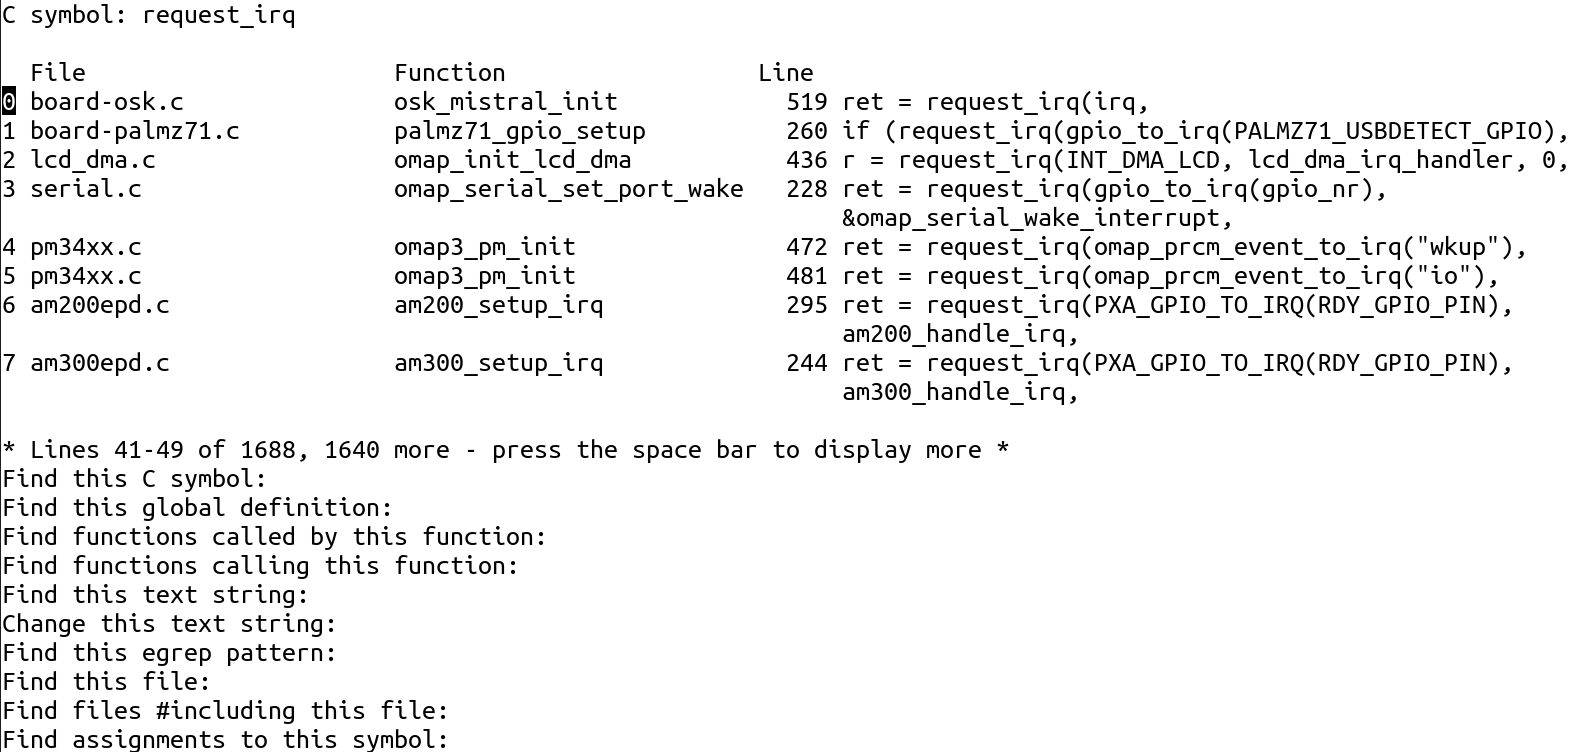
\includegraphics[width=\textwidth]{slides/kernel-source-code-management/cscope.png}
  \end{center}
\end{frame}

\begin{frame}
  \frametitle{LXR: Linux Cross Reference}
  \begin{itemize}
  \item \url{http://sourceforge.net/projects/lxr}
  \item Generic source indexing tool and code browser
    \begin{itemize}
    \item Web server based, very easy and fast to use
    \item Very easy to find the declaration, implementation or usages
      of symbols
    \item Supports C and C++
    \item Supports huge code projects such as the Linux kernel (431 MB
      of source code in version 3.0).
    \item Takes a little time and patience to setup (configuration,
      indexing, server configuration) but indexing a new version is
      quite fast (20 minutes)
    \item You don't need to set up LXR by yourself. Use our
      \url{http://lxr.free-electrons.com} server!
    \end{itemize}
  \end{itemize}
\end{frame}

\begin{frame}
  \frametitle{LXR screenshot}
  \begin{center}
    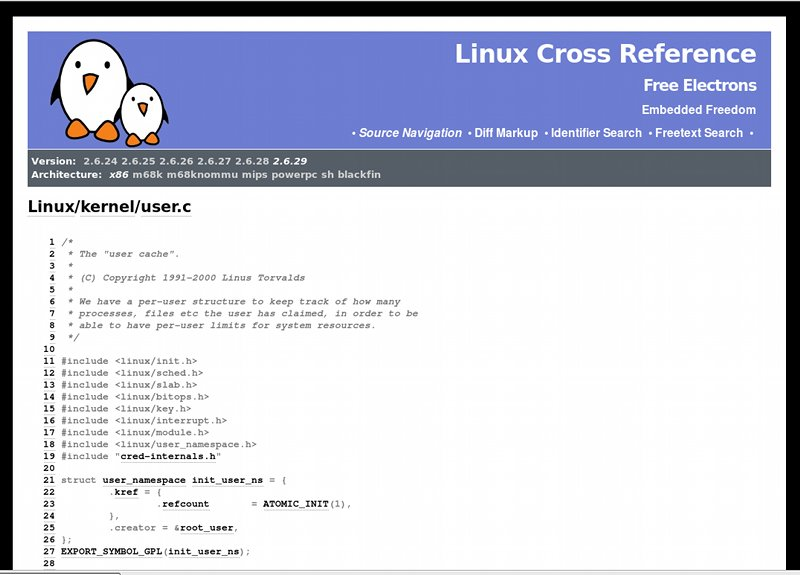
\includegraphics[width=\textwidth]{slides/kernel-source-code-management/lxr.png}
  \end{center}
\end{frame}

